\documentclass[informe.tex]{subfiles}
\begin{document}
  
  \section{Resultados}
    Para analizar los distintos métodos decidimos generar 9 folds con los datos. Teniendo un conjunto provisto es de 900 datos, cada entrenamiento se realiz\'o con 800 entradas y la validación con las 100 restantes. Además, cada experimento fue repetido 5 veces a fin de tener diferentes corridas de cada caso y observar si se produc\'ian diferentes resultados con cada una.
    
    \subsection{Reducción de dimensiones}
      Para analizar este modelo se consideraron los dos criterios de parada mencionados anteriormente: componentes principales ortogonales y $\Delta W$ nulo. Para cada una de esas opciones se usaron las reglas de Oja y de Sanger de modo de poder probar las distintas combinaciones y comparar sus resultados. 
      
      ~
      
      En cada experimento se realizó un gráfico en el cual cada instancia se indica en un espacio tridimensional correspondiente a las tres componentes principales con diferentes colores según la clase. Allí, cada clase de entre las posibles (1 al 9) recibe un color y las instancias de entrenamiento son representadas con un círculo mientras que las de validación se indican con un triángulo. El objetivo entonces es observar cuál es la distribución de las instancias en ese espacio.
      
      ~
      
      El l\'imite de cantidad de \'epocas elegido fue $500$ considerando que es un n\'umero lo suficientemente grande para que el método converja. En todos los casos, si no se llega a que los vectores sean ortogonales o bien que $\Delta W$ sea pequeño entonces el criterio de corte es alcanzar ese límite máximo de épocas. Además, el valor de epsilon elegido fue $0.001$.

      \subsubsection{Resumen de resultados}
      
	En todos los casos 
	\begin{itemize}
	\item $A$ es ``Cantidad de veces con corte por máximo de épocas''
	\item $B$ es ``Cantidad de veces con corte por ortogonalidad''
	\item $C$ es ``Corte por épocas error mínimo''
	\item $D$ es ``Corte por épocas error máximo''
	\item $E$ es ``Corte por épocas error promedio''
	\item $F$ es ``Corte por ortogonalidad cantidad de épocas mínima''
	\item $G$ es ``Corte por ortogonalidad cantidad de épocas máxima''
	\item $H$ es ``Corte por ortogonalidad cantidad de épocas promedio''
	\end{itemize}
  
	
	
	\begin{table}[H]
	  \centering
	  \begin{tabular}{|l|l|l|l|l|l|l|l|l|} \hline
	  Fold & $A$ & $B$ & $C$ & $D$ & $E$ & $F$ & $G$ & $H$ \\ \hline
	  1& 1 & 0 & 0.004782 & 0.004782 & 0.004782 & -- & -- & -- \\ \hline
	  2& 1 & 0 & 0.004761 & 0.004761 & 0.004761 & -- & -- & -- \\ \hline
	  3& 1 & 0 & 0.004757 & 0.004757 & 0.004757 & -- & -- & -- \\ \hline
	  4& 1 & 0 & 0.003081 & 0.003081 & 0.003081 & -- & -- & -- \\ \hline
	  5& 0 & 1 & -- & -- & -- & 15 & 15 & 15 \\ \hline
	  6& 1 & 0 & 0.004767 & 0.004767 & 0.004767 & -- & -- & -- \\ \hline
	  7& 0 & 1 & -- & -- & -- & 13 & 13 & 13 \\ \hline
	  8& 1 & 0 & 0.004777 & 0.004777 & 0.004777 & -- & -- & -- \\ \hline
	  9& 0 & 1 & -- & -- & -- & 5 & 5 & 5 \\ \hline
	  \end{tabular}
	  \caption{Resultados para los 9 folds, usando ortogonalidad como criterio de parada y usando la regla de Sanger. Las cantidades y promedios son sobre todas las repeticiones hechas.}
	  \label{tab:ortogonalidad_sanger}
	\end{table}

	
	\begin{table}[H]
	  \centering
	  \begin{tabular}{|l|l|l|l|l|l|l|l|l|} \hline
	  Fold & $A$ & $B$ & $C$ & $D$ & $E$ & $F$ & $G$ & $H$ \\ \hline
	  1& 0 & 1 & -- & -- & -- & 27 & 27 & 27 \\ \hline
	  2& 0 & 1 & -- & -- & -- & 25 & 25 & 25 \\ \hline
	  3& 0 & 1 & -- & -- & -- & 27 & 27 & 27 \\ \hline
	  4& 0 & 1 & -- & -- & -- & 10 & 10 & 10 \\ \hline
	  5& 0 & 1 & -- & -- & -- & 27 & 27 & 27 \\ \hline
	  6& 0 & 1 & -- & -- & -- & 27 & 27 & 27 \\ \hline
	  7& 0 & 1 & -- & -- & -- & 24 & 24 & 24 \\ \hline
	  8& 0 & 1 & -- & -- & -- & 25 & 25 & 25 \\ \hline
	  9& 0 & 1 & -- & -- & -- & 1 & 1 & 1 \\ \hline
	  \end{tabular}
	  \caption{Resultados para los 9 folds, usando ortogonalidad como criterio de parada y usando la regla de Oja. Las cantidades y promedios son sobre todas las repeticiones hechas.}
	  \label{tab:ortogonalidad_oja}
	\end{table}

	
	\begin{table}[H]
	  \centering
	  \begin{tabular}{|l|l|l|l|l|l|l|l|l|} \hline
	  Fold & $A$ & $B$ & $C$ & $D$ & $E$ & $F$ & $G$ & $H$ \\ \hline
	  1& 0 & 0 & -- & -- & -- & -- & -- & -- \\ \hline
	  2& 0 & 0 & -- & -- & -- & -- & -- & -- \\ \hline
	  3& 0 & 0 & -- & -- & -- & -- & -- & -- \\ \hline
	  4& 0 & 0 & -- & -- & -- & -- & -- & -- \\ \hline
	  5& 0 & 0 & -- & -- & -- & -- & -- & -- \\ \hline
	  6& 0 & 0 & -- & -- & -- & -- & -- & -- \\ \hline
	  7& 0 & 0 & -- & -- & -- & -- & -- & -- \\ \hline
	  8& 0 & 0 & -- & -- & -- & -- & -- & -- \\ \hline
	  9& 0 & 0 & -- & -- & -- & -- & -- & -- \\ \hline
	  \end{tabular}
	  \caption{Resultados para los 9 folds, usando $\Delta W$ como criterio de parada y usando la regla de Sanger. Las cantidades y promedios son sobre todas las repeticiones hechas.}
	  \label{tab:pesos_sanger}
	\end{table}      
	

	\begin{table}[H]
	  \centering
	  \begin{tabular}{|l|l|l|l|l|l|l|l|l|} \hline
	  Fold & $A$ & $B$ & $C$ & $D$ & $E$ & $F$ & $G$ & $H$ \\ \hline
	  1& 0 & 0 & -- & -- & -- & -- & -- & -- \\ \hline
	  2& 0 & 0 & -- & -- & -- & -- & -- & -- \\ \hline
	  3& 0 & 0 & -- & -- & -- & -- & -- & -- \\ \hline
	  4& 0 & 0 & -- & -- & -- & -- & -- & -- \\ \hline
	  5& 0 & 0 & -- & -- & -- & -- & -- & -- \\ \hline
	  6& 0 & 0 & -- & -- & -- & -- & -- & -- \\ \hline
	  7& 0 & 0 & -- & -- & -- & -- & -- & -- \\ \hline
	  8& 0 & 0 & -- & -- & -- & -- & -- & -- \\ \hline
	  9& 0 & 0 & -- & -- & -- & -- & -- & -- \\ \hline
	  \end{tabular}
	  \caption{Resultados para los 9 folds, usando $\Delta W$ como criterio de parada y usando la regla de Oja. Las cantidades y promedios son sobre todas las repeticiones hechas.}
	  \label{tab:pesos_oja}
	\end{table}            

	
      \subsubsection{Gráficos espaciales de algunos resultados}
	\newgeometry{textwidth=21cm,textheight=21cm}
	\begin{figure}[H]
        \centering
        \begin{subfigure}[b]{0.49\textwidth}
                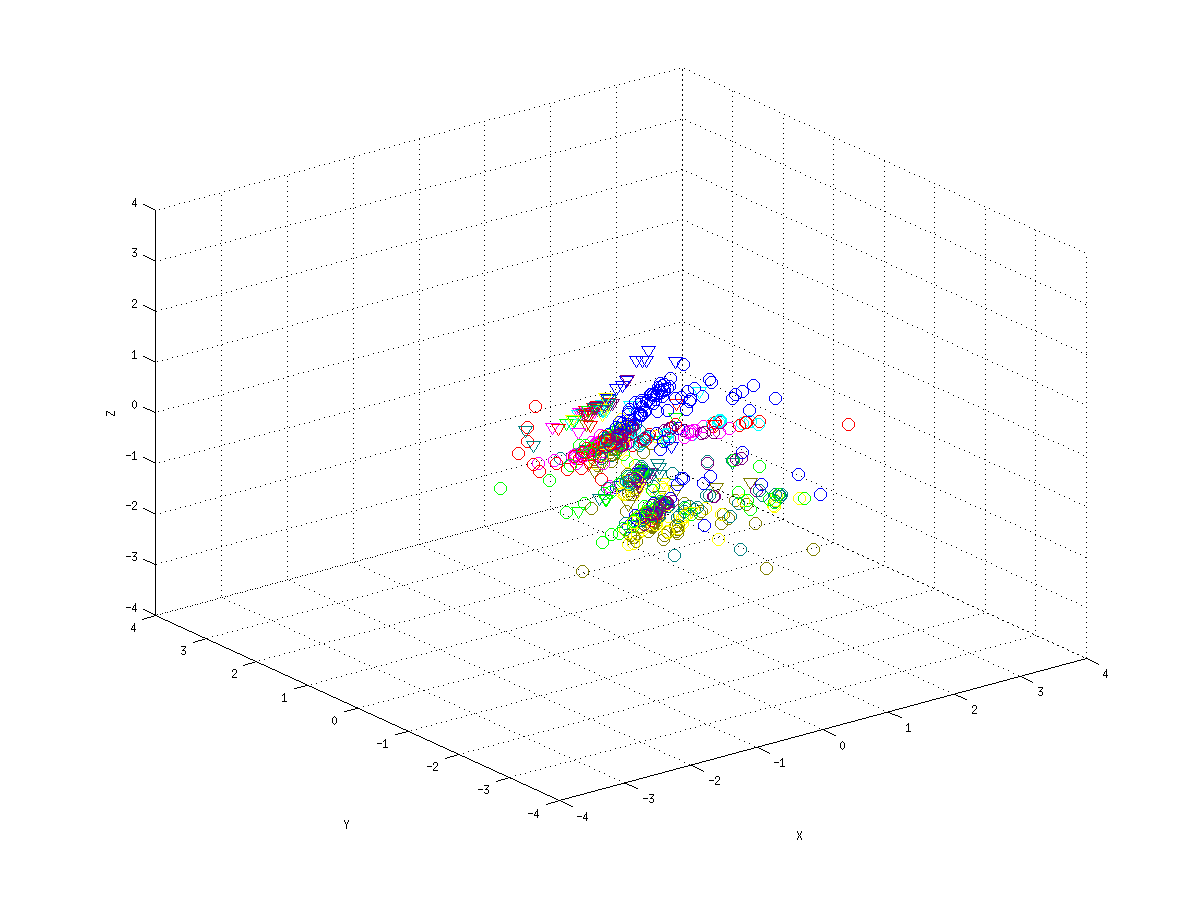
\includegraphics[width=\textwidth]{graficos/fold1_criterioParadao_reglaM_alpha0_rep1_0P.png}
                \caption{Vista en perspectiva.}
        \end{subfigure}%
        ~ %add desired spacing between images, e. g. ~, \quad, \qquad, \hfill etc.
          %(or a blank line to force the subfigure onto a new line)
        \begin{subfigure}[b]{0.49\textwidth}
                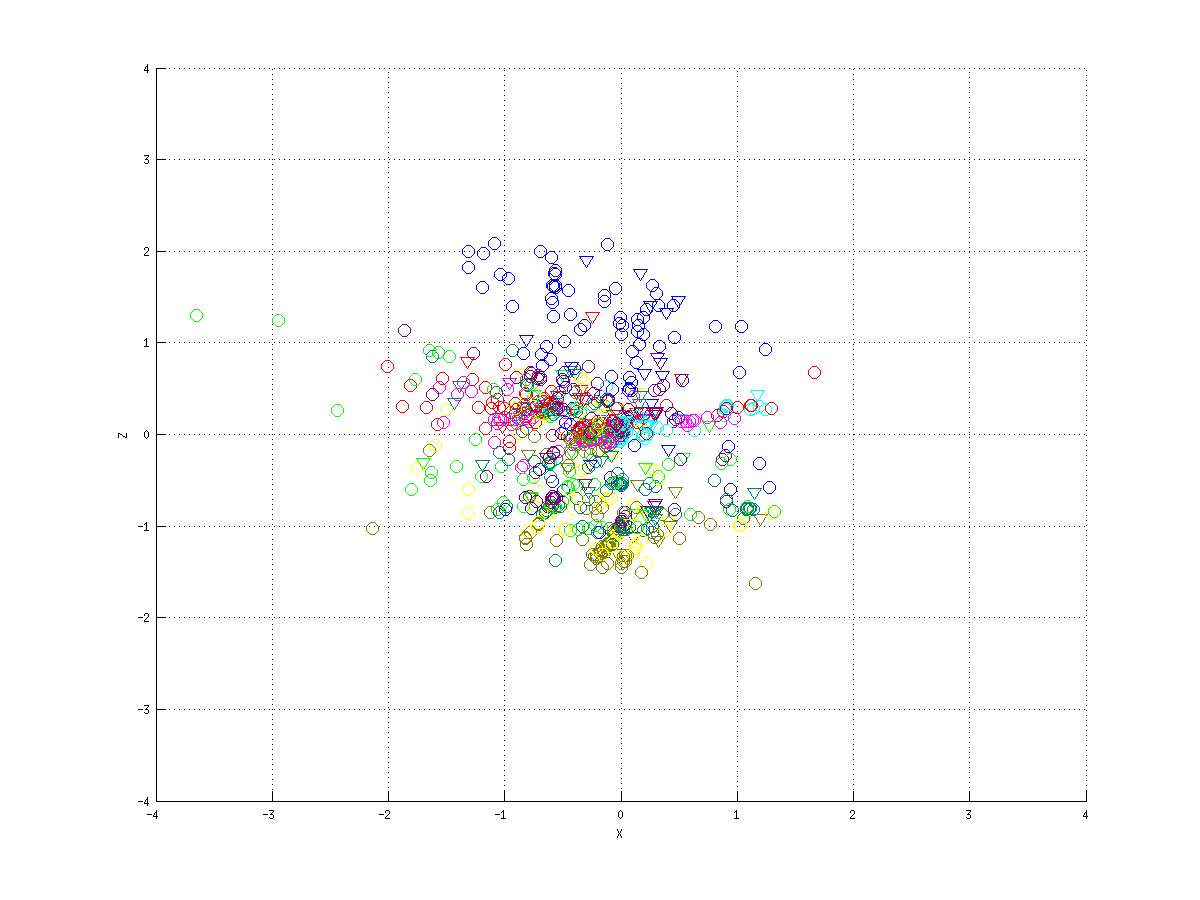
\includegraphics[width=\textwidth]{graficos/fold1_criterioParadao_reglaM_alpha0_rep1_1XZ.png}
                \caption{Plano X-Z.}
        \end{subfigure}
        
        \begin{subfigure}[b]{0.49\textwidth}
                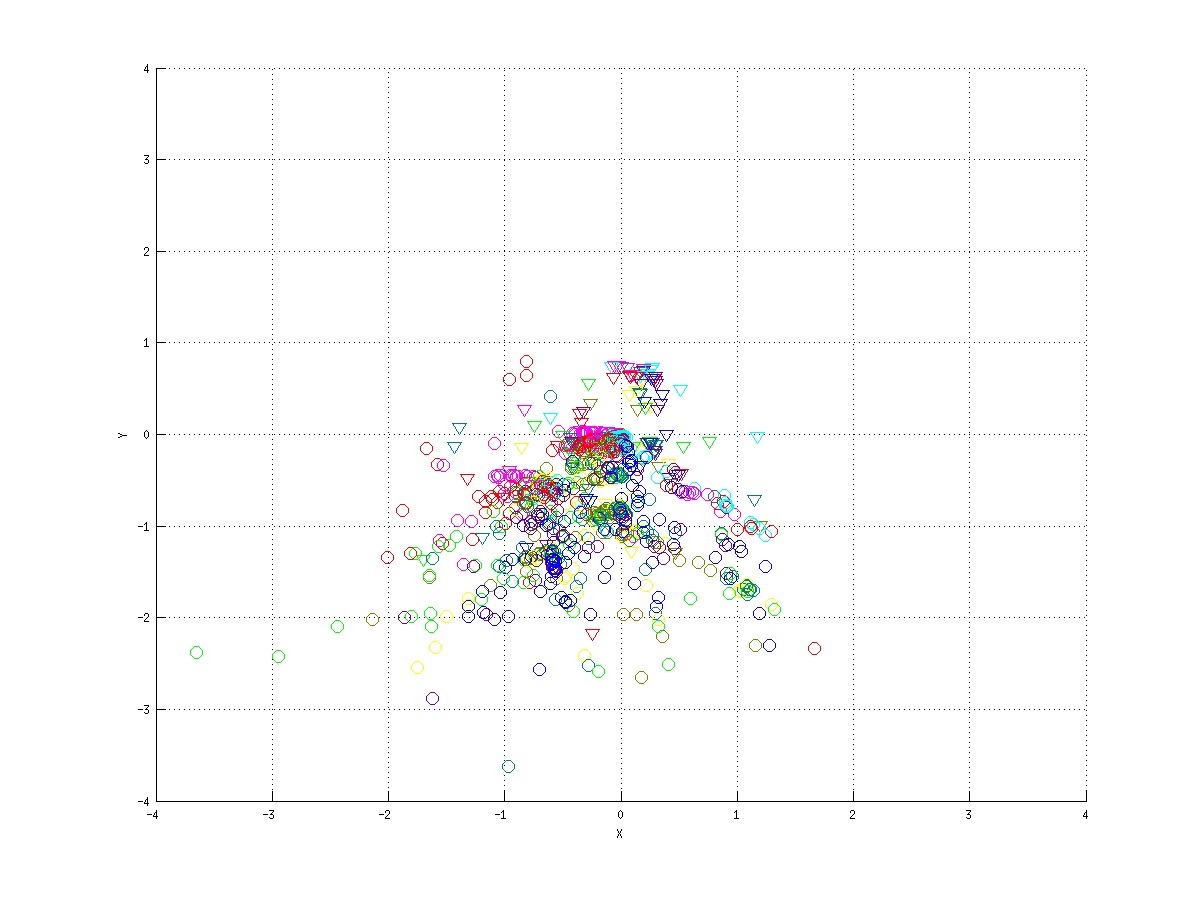
\includegraphics[width=\textwidth]{graficos/fold1_criterioParadao_reglaM_alpha0_rep1_2XY.png}
                \caption{Plano X-Y.}
        \end{subfigure}
        ~ %add desired spacing between images, e. g. ~, \quad, \qquad, \hfill etc.
          %(or a blank line to force the subfigure onto a new line)
        \begin{subfigure}[b]{0.49\textwidth}
                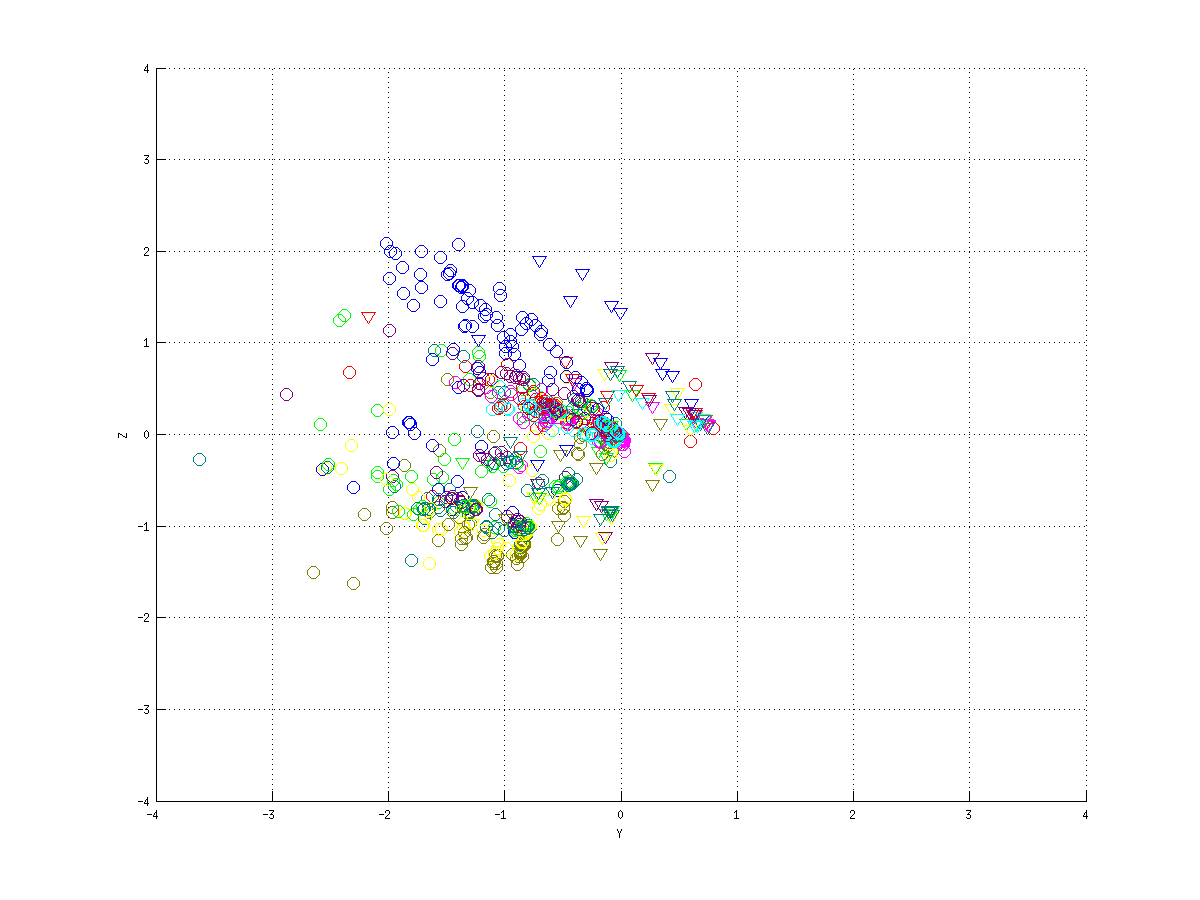
\includegraphics[width=\textwidth]{graficos/fold1_criterioParadao_reglaM_alpha0_rep1_3YZ.png}
                \caption{Plano Y-Z.}
        \end{subfigure}
        \caption{Gráfico espacial para blablabla}
        \label{fig:blablabla}
	\end{figure}
      
	\restoregeometry
      
      
      
    \subsection{Mapeo de características}
    
      En este caso, el analisis de este modelo se vuelve algo particular. Para realizar el mismo, decidimos utilizar dos metricas: la primera con el objetivo de obtener alguna nocion de desempe\~no de la red, y la segunda para conocer que tan distanciados estaban los distintos grupos de activacion luego del entrenamiento.
      
      % TODO: (Para Rober) Explicar que son los dominantes en la seccion de desarrollo.
      
      \subsubsection{Distancia a dominantes}
      
      A la primera la llamaremos ``distancia a dominantes'' (DD) y representar\'a la distancia relativa media entre los dominantes del set de validaci\'on y el set de activaci\'on. Para generar su calculo, tomamos cada uno de los dominantes del mapa de validacion y buscamos el dominante mas cercano en el mapa de entrenamiento, en el mejor caso esta distancia es cero. 
      
      ~
      
      Obteniendo todas las distancias entre los distintos dominantes calcularemos su media y luego la normalizaremos diviendola por la distancia maxima que puede existir; esto es $||(M_1,M_2)||$, es decir la distancia entre las esquinas de la matriz de pesos.
      
      $$DD(DTr, DTe, W, M_1, M_2) = \frac{dM(mAct(DTr,W), mAct(DTe,W))}{||(M_1,M_2)||}$$
      
      Donde $DTr$ es el dataset de entrenamiento, $DTe$ es el dataset de validacion, $W$ es la matriz de pesos y $M_1, M_2$  son las dimensiones de la ultima. Se supone que $mAct$ calcula los mapas de dominantes para los datos otorgados y que $dM$ calcula la distancia media entre dichos dominantes.
      
      \subsubsection{Factor de cruce}
      
      La segunda ser\'a denominada como ``factor de cruce'' (FC) y nos dara una nocion de cuantas neuronas se activan mas de una clase. Esto nos sirve para observar de que forma la red neuronal esta respondiendo a distintos impulsos. Inferimos que es deseable que este factor sea bajo, ya que lo ideal seria que las distintas clases activen grupos de neuronas disjuntas.
      
      ~
      
      Para calcular este factor, nos armaremos un mapa de la red neuronal en donde tendremos registradas las cantidades de veces que se activo una neurona en las 9 clases distintas. En un escenario ideal, ningun numero deberia ser mayor a 1, ya que indicaria que una neurona se activo para mas de una clase.
      
      ~
      
      Una vez calculado este mapa sumaremos todos los valores de la matriz, le restaremos la cantidad de neuronas que no eran cero dentro del mapa (por lo que en el caso ideal el factor nos daria cero) y lo dividiremos por esa misma cantidad.
      
      $$FD(D, W) = \frac{sumActCruz(D, W) - noSonCero(D, W)}{noSonCero(D, W)}$$
      
      Donde $D$ representa los datos a utilizar y $W$ la matriz de pesos de la red neuronal ya entrenada. Se supone que $sumActCruz$ internamente calcula las activaciones, al igual que $noSonCero$ calcula la cantidad de neuronas que se activaron.
      
      ~
      \subsubsection{Analisis de resultados}
      Analizar los resultados de las metricas decidimos generar 9 folds distintos para luego promediar los resultados de los mismos. Cada fold tendra un set de entrenamiento y uno de validación generados al azar.
    
      %Para realizar el modelo se consideraron distintos tamaños de mapa así como también la opción de tener parámetros de aprendizaje autoajustables. El objetivo es tener un criterio comparativo para determinar qué tamaño es suficiente en relación a la cantidad de parámetros de las instancias.
      
      %Por otro lado, una vez generados los mapas con el conjunto de entrenamiento, el objetivo es catalogar las instancias del conjunto de validación usando los pesos y el mapa entrenados. 
      

\end{document}